\chapter{Circles}

A circle is the set of points $(x, y)$ that are a particular distance $r$ from a
particular point $(x_c, y_c)$.  We say that $r$ is the
\newterm{radius} and $(x_c, y_c)$ is the \newterm{center}

\begin{center}
\begin{tikzpicture}
    \filldraw [sdkblue] (1,2) circle (2pt) node[anchor=west]{$(x_c, y_c)$};
    \filldraw [sdkblue] (2,4.82842712474619) circle (2pt) node[anchor=west]{
    $(x, y)$};
    \draw [sdkblue,dashed](1,2) -- (2,4.82842712474619) node[midway,anchor=
    west] {$r$};
    \draw [sdkblue](1,2) circle (3);
    \draw [stealth-stealth](-2.5,0)--(4.5,0);
    \draw [stealth-stealth](0,-1.5)--(0,5.5);
\end{tikzpicture}
\end{center}


\begin{mdframed}[style=important, frametitle={Area and Radius}]

  If the radius of a circle is $r$, the area of its interior ($a$) is given 
  by \index{circle!area of}

  $$a = \pi r^2$$

\end{mdframed}

\begin{Exercise}[title={Area of a Circle}, label=area_of_circle]

  The paint you have says ``One liter covers 6 square meters.''

  You are painting the top of a circular table with a radius of 3 meters.

  How much paint will you need?
  
\end{Exercise}
\begin{Answer}[ref=area_of_circle]

  The table has a radius of 3 meters.

  So the area of its top is $3^2 \pi \approx 28.27$.

  $$ 28.27 \text{ square meters }\left(\frac{1 \text{ liter }}{6 \text{ square 
  meters }} \right) = 4.72 \text{ liters }$$ 
  
\end{Answer}


Note that a circle lives in a particular plane. The points $(x, y, z)$ that 
are a particular distance $r$ from a particular point $(x_c, y_c, z_c)$ are a 
sphere:

\begin{center}
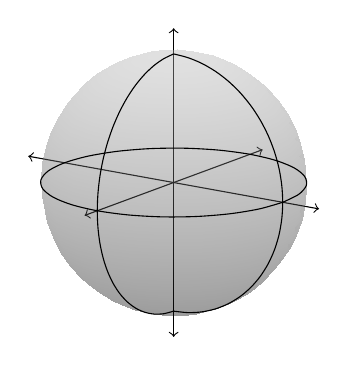
\begin{tikzpicture}
  \begin{axis}[
    view={35}{15},
    unit vector ratio=1 1 1,
    ticks = none,
    axis lines=middle,
    ymin=-3.5,
    ymax=3.5,
    xmax=4.0,
    xmin=-4.0,
    zmin=-3.6,
    zmax=3.6,
    x axis line style=<->,
    y axis line style=<->,
    z axis line style=<->,
    clip=false
    ]
    \addplot3[surf,shader=interp,domain=0:360,y domain=-90:90, opacity=0.4,
    colormap={blackwhite}{color=(black) color=(black!30)}] ({3 * cos(y) * 
    cos(x)},
    {3 *  cos(y) * sin(x)},{3 * sin(y)});
    \addplot3[samples y=0,domain=0:360,smooth]({3*cos(x)}, {3*sin(x)}, 0.0);
    \addplot3[samples y=0,domain=-180:0,smooth](0, {3*sin(x)}, {3*cos(x)});
    \addplot3[samples y=0,domain=0:180,smooth]({3*sin(x)}, 0, {3*cos(x)});
  \end{axis}
\end{tikzpicture}
\end{center}


The distance all the way across the middle of a circle (or a sphere) is its
\newterm{diameter}.  The diameter is always twice the radius.

For the rest of the chapter, we are talking about circles, points, and
lines \textit{in a plane}.

\begin{mdframed}[style=important, frametitle={Circumference and Diameter}]

  The circumference ($c$) of a circle is the distance around the circle. If the
  diameter is $d$, \index{circumference}

  $$c = \pi d$$

\end{mdframed}

\begin{Exercise}[title={Circumference}, label=circumference]

  Using a tape measure, you figure out that the circumference of a tree in your
  yard is 64 cm.

  Assuming the trunk is basically circular,  what is its diameter?
  
\end{Exercise}
\begin{Answer}[ref=circumference]

  The diameter is $$\frac{c}{\pi} = \frac{64}{\pi} \approx 20.37 \text{ 
  centimeters}$$
  
\end{Answer}
\begin{Exercise}[title={Splitting a Pie}, label=pie_splitting]

  A pie has a radius of 13 cm.  7 friends all want equal sized wedges.  You 
  have a tape measure.

  How many centimeters will each outer crust be?

\end{Exercise}
\begin{Answer}[ref=pie_splitting]

  The circumference of the pie is $26 \pi \approx 81.7$ centimenters.
  
  The length of the crust for each piece would be about $\frac{81.7}{7} = 11.7$
  cm.

  
\begin{tikzpicture}
    \filldraw [black] (0,0) circle (2pt);
    \draw [black](0,0) circle (3);
    \foreach \x in {0,...,6}
    \draw [dashed] (0,0) -- ({3 * cos(\x * 51.428571428571429)}, {3 * sin(\x 
    * 51.428571428571429)});
    \draw [sdkblue,very thick] (3, 0) arc (0:51.43:3) node [midway, anchor=east] 
    {11.7 cm};
    \node at (1.0, 1.5)  {13 cm};
\end{tikzpicture}
\end{Answer}

\section{Arc Length}
Previously, you learned that angles can be measured in degrees and radians. A 
circle is $360^o$ (see figure \ref{fig:circledeg}). 

\begin{figure}[htbp]
\centering
\begin{tikzpicture}
        \begin{polaraxis}[axis lines = none, clip = false]
    \draw[black](0,0) -- (0, 3);
    \draw[black, dashed] (0,0) -- (180, 3);
    \addplot[blue, thick, domain = 0:360, samples = 200]{2.5};
    \addplot[red, domain = 0:175]{1};
    \draw[red, -latex](175, 1) -- (180,1);
    \addplot[red, domain = 180:355]{1};
    \draw[red, -latex] (355, 1) -- (360, 1);
    \node[] at (90, 1.5) {$\theta_1 = 180^\circ$};
    \node[] at (270, 1.5) {$\theta_2 = 180^\circ$};
    \end{polaraxis}
    \end{tikzpicture}
    \caption{The total internal angle of a circle is $\theta_1 + \theta_2 = 
    360^\circ$}
    \label{fig:circledeg}
\end{figure}

This means a circle is also $2\pi$ radians:
$$360^\circ \cdot \frac{\pi}{180^\circ} = 2\pi$$

You may have been wondering: why is it that there are $\pi$ radians in a 
$180^\circ$ angle? A radian is defined such that one radian is the angle at the 
center of a circle which defines an arc of the circumference equal to the 
radius of the circle (see figure \ref{fig:oneradian}). 

\begin{figure}[htbp]
\centering
\begin{tikzpicture}
        \begin{polaraxis}[axis lines = none, ymin = 0, ymax = 3, 
	clip = false]
 \addplot[blue, thick, domain = 0:360, samples = 300] {2.5};
 \addplot[red, thick, domain = 0:57.3] {2.5};
 \draw[red, thick](0,0) -- (0, 2.5);
 \draw[red, thick] (0,0) -- (57.3, 2.5);
 \addplot[red, domain = 0:57.3]{0.5};
 \addplot[black, domain = 0:57.3]{2.75};
 \draw[black](0,2.7) -- (0,2.8);
 \draw[black] (57.3, 2.7) -- (57.3, 2.8);
 \node[rotate = -60] at (27.5, 2.9) {\small length $= r$};
 \node[] at (27.5, 1) {\small $\theta = 1$};
    \end{polaraxis}
    \end{tikzpicture}
    \caption{When the center angle is 1 radian, the length of the arc is equal 
    to the radius of the circle}
    \label{fig:oneradian}
\end{figure} 



This makes it very straightforward to find the lengths of arcs if we know the 
center angle in radians. The arc length is just $r \theta$, where $\theta$ is 
the center angle in radians. 

\begin{mdframed}[style=important, frametitle={Length of an Arc}]

If you have two points $a$ and $b$ on a circle, the ray from the
center through $a$ and the ray from the center through $b$ form an
angle.  If $\theta$ is the angle in radians and $r$ is the radius of
the circle, the distance from $a$ to $b$ on the circle is $r \theta$.

\begin{center}
\begin{tikzpicture}
    \filldraw [black] (0,0) circle (2pt) node[anchor=west]{Center};
    \filldraw [sdkblue] (-1,2.82842712474619) circle (2pt) node[anchor=west]{$b$};
    \filldraw [sdkblue] (2.12132,2.12132) circle (2pt) node[anchor=east]{$a$};
    \draw [sdkblue,dashed,->](0,0) -- (-1.2,3.394112549695428);
    \draw [sdkblue,dashed,->](0,0) -- (2.4, 2.4) node[midway,anchor=east]{$r$};
    \draw [black](0,0) circle (3);
    \draw [sdkblue,very thick] (2.12132,2.12132) arc (45:109.47:3) node [midway, 
    anchor=south] {$r \theta$};
    \draw [sdkblue, <->] (0.707,0.707) arc (45:109.47:1) node [midway, 
    anchor=south]{$\theta$};
\end{tikzpicture}
\end{center}


\end{mdframed}

This shows us why $\pi\text{ radians} = 180^\circ$. Recall the formula for 
circumference: $c = \pi d$, where $d$ is the diameter of the circle. Since the 
diameter is twice the radius, then we can also say that $c = 2\pi r$, where r 
is the radius of the circle. The circumference of the circle is just an arc 
where the central angle is the entirety of the circle. Since we know that the 
length of an arc is $r \theta$, we can find the total internal angle of a 
circle in radians:
$$2 \pi r = r \theta$$
$$\theta = 2\pi$$
Which is how we know $360^\circ = 2\pi\text{ radians}$. 

\begin{Exercise}[title = {Angle of Rotation}, label = radian1]
A car tire has a radius of approximately 25 centimeters. If you roll your car 
forward 10 cm, by how many radians has your tire rotated?
\end{Exercise}

\begin{Answer}[ref = radian1]
If you roll forward by 10 cm, that means you move along the edge of your tire 
such that the arc length is 10 cm. So, we are looking for a central angle such 
that $r \theta = 10 \text{ cm}$. Substituting $r = 25 \text{ cm}$ and solving 
for $\theta$: $\theta = \frac{10\text{ cm}}{25\text{ cm}} = 0.4\text{ radians}$. 
\end{Answer}

\begin{Exercise}[title = {Arc Length Ranking}, label = radian2]
Rank the following arc lengths from longest to shortest (the central angle that defines the arc and the radius of the circle are provided:
\begin{enumerate}
\item central angle of $\frac{\pi}{4}$ and a radius of 2 cm
\item central angle of $\pi$ and a radius of 1 cm
\item central angle of $\frac{\pi}{10}$ and a radius of 5 cm
\item central angle of $\frac{3\pi}{4}$ and a radius of 3 cm
\end{enumerate}
\end{Exercise}

\begin{Answer}[ref = radian2]
\begin{enumerate}
\item $\frac{\pi}{4} \cdot 2\text{ cm} = \frac{\pi}{2}\text{ cm}$
\item $\pi \cdot 1\text{ cm} = \pi \text{ cm}$
\item $\frac{\pi}{10} \cdot 5\text{ cm} = \frac{\pi}{2}\text{ cm}$
\item $\frac{3\pi}{4} \cdot 3\text{ cm} = \frac{9\pi}{4}\text{ cm}$
\end{enumerate}
Therefore, from longest to shortest are 4, (1,3), 2 (1 and 3 are the same length).
\end{Answer}

\begin{Exercise}[title={Arc Length}, label=arc_length]

You have been asked to find the radius of a very large cylindrical tank.
You have a tape measure, but it is only 15 meters long and doesn't
reach all the way around the tank.

However, you have a compass.  So you stick one end of the tape measure
to the side of the tank and measure the orientation of the wall at
that point.  Then you walk the 15 meters and measure the orientation of the 
wall there.

You find that 15 meters represents 72 degrees of arc.

What is the radius of the tank in meters?
  
\end{Exercise}
\begin{Answer}[ref=arc_length]

  $$72 \text{ degrees } \left(\frac{2\pi \text{ radians }}{360 \text{ degrees }
  }\right) \approx 1.2566 \text{ radians }$$

  $$15 = 1.2566r$$

  $$r = 11.94 \text{ meters}$$
  
\begin{tikzpicture}
    \filldraw [black] (0,0) circle (2pt);
    \draw [black](0,0) circle (3);
    \draw [dashed] (0,0) -- ({3 * cos(72)}, {3 * sin(72)});
    \draw [dashed] (0,0) -- (3, 0);
    \draw [sdkblue,very thick] (3,0) arc (0:72:3) node [midway, anchor=east] 
    {15 m};
    \draw [sdkblue, <->] (1,0) arc (0:72:1) node [midway, anchor=east]{$72^
    \circ$ = 1.2566 rad};
    \node at (0.0, 1.6)  {11.94 m};
\end{tikzpicture}
\end{Answer}

\section{Sector Area}
We already know the area of a circle is given by $A = \pi r^2$. What about a 
piece of a circle? Let's start with a straightforward example:

\textbf{Example}: A pizza with a radius of $15$ cm is divided into 6 equal 
pieces. What is the area of each piece?

\textbf{Solution}: First, we find the area of the entire pizza:
$$A = \pi r^2$$
$$A = \pi (18\text{ cm})^2$$
$$A = 324\pi\text{ cm}^2 \approx 1018\text{ cm}^2$$

Then, we divide by 6, since the pieces of equal sizes:
$$A_{piece} = \frac{A}{6} = \frac{324\pi\text{ cm}^2}{6} = 54\pi\text{ cm}^2$$

Let's use this to write a general formula for the area of a sector defined by a 
central angle $\theta$ (see figure \ref{fig:wedge}). We know that when a 
circle is divided into 6 equal sectors, the central angle of each wedge is 
$\theta = \frac{2\pi}{6} = \frac{\pi}{3}$. Additionally, we know the area of 
each wedge is the total area divided by 6: $A_{sector} = \frac{\pi r^2}{6} = 
\frac{\pi}{6} r^2 = \frac{\theta}{2} r^2$. 

\begin{mdframed}[style=important, frametitle={Area of a Wedge}]
For a sector whose corner is at the center of a circle, the area is given by 
$A_{sector} = \frac{\theta}{2} r^2$, where $\theta$ is the central angle and $r$ is the radius. 

\end{mdframed}

\begin{figure}[htbp]
\centering
\begin{tikzpicture}
        \begin{polaraxis}[axis lines = none, ymin = 0, ymax = 3, 
	clip = false]
 \addplot[blue, thick, domain = 0:360, samples = 300] {2.5};
 \addplot[name path= arc, red, thick, domain = 0:135] {2.5};
 \addplot[name path= legs, red, thick] coordinates {(135, 2.5) (135, 0) (0, 0) (0, 2.5)};
 \addplot[red!30, opacity = 0.4] fill between [of=arc and legs];
 \addplot[red, domain = 0:135]{0.5};
 \node[] at (50, 0.75) {\small $\theta$};
    \end{polaraxis}
    \end{tikzpicture}
    \caption{The area of a sector with central angle $\theta$ is $\frac{\theta}{2}r^2$}
    \label{fig:wedge}
\end{figure}

\begin{Exercise}[title = {Area of a Wedge}, label = wedge]
You are tasked with painting a large, circular logo on the side of a building. 
If a liter of paint covers covers 6 square meters and the logo is 5 meters 
wide, how many liters of red paint will you need to paint a wedge whose central 
angle is $\frac{3\pi}{4}$ radians?
\end{Exercise}

\begin{Answer}[ref = wedge]
If the logo is 5 meters wide, the diameter is 5 meters and the radius is 2.5 
meters. Using the formula for the area of a wedge: $A_{wedge} = \frac{1}{2}
\frac{3\pi}{4}(21.5\text{ m})^2 \approx 7.363\text{ m}^2$. Since a liter covers 
$6\text{ m}^2$, you will need $\frac{7.363}{6} \approx 1.227\text{ L}$ of paint. 
\end{Answer}

\section{Tangents}

A line that is \newterm{tangent}\index{tangent line} to a circle touches it at 
exactly one point:

\begin{tikzpicture}
    \filldraw [black] (0,0) circle (2pt);
    \draw [dashed, black](0,0) circle (3);
    \filldraw [sdkblue] (2.121, 2.121) circle (2pt);
    \draw [sdkblue, thick] (6.243, -2) -- (0, 4.243);
\end{tikzpicture}

The tangent line is always perpendicular to the radius to the point of tangency:

\begin{tikzpicture}
  \filldraw [black] (0,0) circle (2pt);
  \draw [dashed, black](0,0) circle (3);
  \filldraw [sdkblue] (2.121, 2.121) circle (2pt);
  \draw [sdkblue, thick] (0,0) -- (2.121, 2.121);
  \draw [black] (1.9, 1.9) -- (2.121, 1.679) -- (2.342,1.9);
  \draw [sdkblue, thick] (6.243, -2) -- (0, 4.243);
\end{tikzpicture}


\begin{Exercise}[title={Painting a Comet}, label=painting_comet]
  
  You have been asked to paint a comet and its tail in yellow on the floor of a 
  gymnasium.

  A liter of yellow paint covers 6 square meters.

  First you draw a circle with a radius of 3 meters.  Then you mark a
  point $D$ on the floor 7 meters from the center of the circle.  Then
  you draw two tangent lines that pass through $D$.

  You use a protractor to measure the angle at which the tangent lines meet: about 
  $51^\circ$
  
  \begin{tikzpicture}
    \filldraw [sdkblue] (0,0) circle (2pt);
    \filldraw [black] (7,0) circle (2pt);
    \draw [sdkblue,dashed] (0,0) -- (3,0) node [midway, anchor=south] {3 m};
    \draw [sdkblue,dashed] (3,0) -- (7,0) node [midway, anchor=south] {4 m};
    \draw [sdkblue,dashed, ->] (5.5,0) arc (180:154.6:1.5) node [midway, 
    anchor=west]{$51^\circ$};
    \draw [sdkblue,dashed, ->] (5.5,0) arc (180:205.4:1.5);
    \draw [black,thick] (7,0) -- ({3 * cos(64.62)}, {3 * sin(64.62)});
    \draw [black,thick] (7,0) -- ({3 * cos(-64.62)}, {3 * sin(-64.62)});
    \filldraw [black] ({3 * cos(64.62)}, {3 * sin(64.62)}) circle (2pt);
    \filldraw [black] ({3 * cos(-64.62)}, {3 * sin(-64.62)}) circle (2pt);
    \filldraw [sdkblue] (3, 0) circle (2pt);
    \draw [sdkblue,dashed] ({3 * cos(-64.62)}, {3 * sin(-64.62)}) arc 
    (-64.62:64.62:3);
    \draw [black,thick] ({3 * cos(64.62)}, {3 * sin(64.62)}) arc 
    (64.62:295.38:3);
  \end{tikzpicture}

  Before you paint the area contained by the circle and the two
  tangent lines, how much paint will you need?
    

\end{Exercise}
\begin{Answer}[ref=painting_comet]

  The trick here is to take advantage of the fact that the tangent is 
  perpendicular to the radius to make right triangles:

  \begin{tikzpicture}
    \coordinate (a) at ({3 * cos(64.62)}, {3 * sin(64.62)});
    \coordinate (b) at ({3 * cos(-64.62)}, {3 * sin(-64.62)});
    \filldraw [sdkblue] (0,0) circle (2pt);
    \filldraw [black] (7,0) circle (2pt);
    \draw [black,thick] (0,0) -- (a) node [midway, anchor=east] {3m};
    \draw [black,thick] (0,0) -- (b) node [midway, anchor=east] {3m};
    \draw [black,thick] (0,0) -- (7,0) node [midway, anchor=south] {7 m};
    \draw [sdkblue,dashed, <->] (5.5,0) arc (180:154.6:1.5) node [midway, 
    anchor=west]{$25.5^\circ$};
    \draw [sdkblue,dashed, <->] (5.5,0) arc (180:205.4:1.5) node [midway, 
    anchor=west]{$25.5^\circ$};
    \draw [sdkblue,dashed, <->] (1.5,0) arc (0:64.5:1.5) node [midway, 
    anchor=west]{$64.5^\circ$};
    \draw [sdkblue,dashed, <->] (1.5,0) arc (0:-64.5:1.5) node [midway, 
    anchor=west]{$64.5^\circ$};
    \draw [black,thick] (7,0) -- (a);
    \draw [black,thick] (7,0) -- (b);
    \filldraw [black] (a) circle (2pt);
    \filldraw [black] (b) circle (2pt);
    \draw [black,thick] (a) arc (64.62:295.38:3);
  \end{tikzpicture}

  The wedge has radius 3 and represents $360 - 2(64.5) = 231^\circ \approx 4.03 
  \text{ radians}$.

  We are finding the area of this piece:
  
  \begin{tikzpicture}
    \coordinate (a) at ({3 * cos(64.62)}, {3 * sin(64.62)});
    \coordinate (b) at ({3 * cos(-64.62)}, {3 * sin(-64.62)});
    \filldraw [sdkblue] (0,0) circle (2pt);
    \draw [black,thick] (0,0) -- (a) node [midway, anchor=west] {3m};
    \draw [black,thick] (0,0) -- (b);
    \draw [sdkblue,dashed, <->] ({1.5 * cos(64.62)}, {1.5 * sin(64.62)}) arc 
    (64.5:295.5:1.5) node [midway]{4.03 rad};
    \filldraw [black] (a) circle (2pt);
    \filldraw [black] (b) circle (2pt);
    \draw [black,thick] (a) arc (64.62:295.38:3);
  \end{tikzpicture}

  The area of this piece is $(4.03)(3^2) = 36.27$ square meters.

  If a right triangle has a hypotenuse of 7m and one leg is 3m, the
  other leg is $\sqrt{7^2 - 3^2} = 2 \sqrt{10} \approx 6.3$ m.

    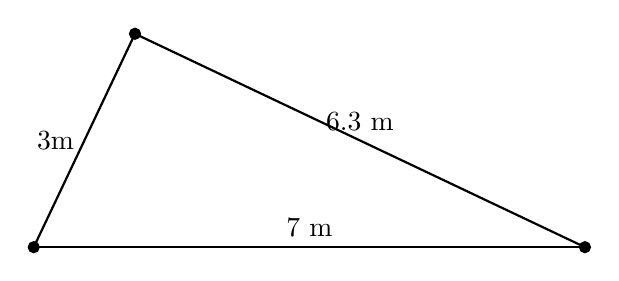
\begin{tikzpicture}
    \coordinate (a) at ({3 * cos(64.62)}, {3 * sin(64.62)});
    \filldraw [black] (7,0) circle (2pt);
    \filldraw [black] (0,0) circle (2pt);
    \draw [black,thick] (0,0) -- (a) node [midway, anchor=east] {3m};
    \draw [black,thick] (0,0) -- (7,0) node [midway, anchor=south] {7 m};
    \draw [black,thick] (7,0) -- (a) node [midway, anchor=south] {6.3 m};
    \filldraw [black] (a) circle (2pt);
  \end{tikzpicture}

  
  A right triangle with legs of 3m and 6.3m has an area of 9.45 square meters.

  There are two of them, so the total area is $36.27 + 2(18.9) = 74.07$ square 
  meters.

  Six square meters per liter, so you need $\frac{74.07}{6} = 12.35$ liters of 
  paint.

\end{Answer}

